% Copyright 2021 Néstor Nápoles López

% This is
% \refsubsubsec{relevanceofpitchspellingtotonalanalysis},
% which introduces the relevance of pitch spelling to tonal
% analysis.

Pitch spelling is likely to be correlated with tonal
analysis. Consider the following example. If during a
musical performance, a pianist presses the key corresponding
to pitch class ``8'' in the piano keyboard (shown in Figure
\ref{fig:Q7_1}), how can we know if the note played by the
performer was an A$\flat$ or a G$\sharp$?\footnote{Assume an
equal-tempered setting, with no special considerations
regarding how the piano might be tuned. That is, the
distinction between the A$\flat$ and G$\sharp$ notes that we
are looking for is of a semantic nature, not of a tuning
nature.}

% \begin{figure}[h] \centering %
% 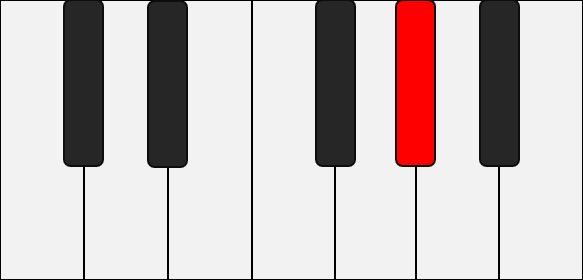
\includegraphics[width=0.6\textwidth]{figures/Q7_1.png} %
% \caption{A note playing in a keyboard. It could be %
% either G$\sharp$ or A$\flat$.} \label{fig:Q7_1} %
% \end{figure}

A first approach could be to determine the spelling of the
note based on the musical key of the piece where the note
was played. Such information can be automatically obtained
using a \gls{gke} model with a reasonable degree of
accuracy. Nevertheless, our pitch-spelling model now
requires information about the key in order to make its
predictions.

The key model could predict that the piece is in, for
example, \emph{A minor}. ``Is it a piece in A minor? Then
the note is probably a G$\sharp$.''

% \begin{figure}[h] \centering %
% 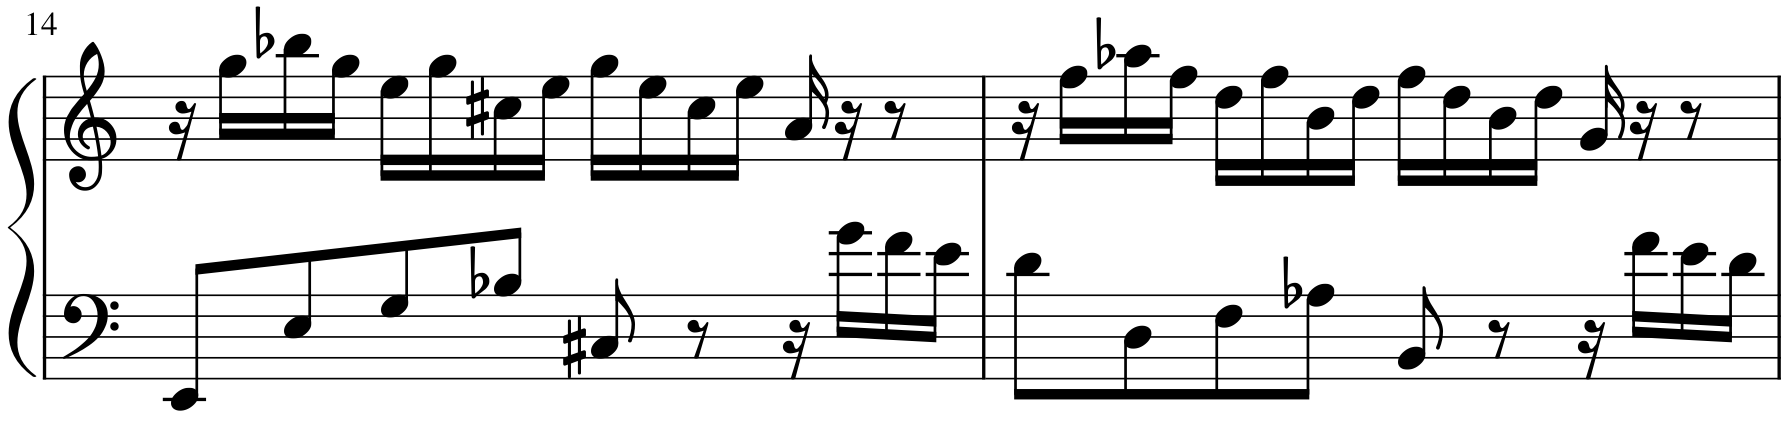
\includegraphics[width=0.8\textwidth]{figures/Q7_2.png} %
% \caption{J. S. Bach's BWV 784, mm. 14-15. The piece is %
% in A minor, however, during measure 15, the pitch % class
% number 8 is spelled as an A$\flat$.} % \label{fig:Q7_2}
% \end{figure}

Figure \ref{fig:Q7_2} shows an adversarial example where the
pitch class number 8 is spelled as A$\flat$ in a piece that
is originally in \emph{A minor}. A person familiarized with
Western tonal music could guess that similar examples as the
one shown in Figure \ref{fig:Q7_2} will occur whenever the
music is modulating or tonicizing a different key.

Assuming that the awareness of modulations and tonicizations
throughout the piece (which we generally refer to as
\emph{local keys}) will mitigate our problems when
predicting the spelling of a note, seems to be a reasonable
guess. Instead of requiring to know the \emph{global key} of
the piece, now, our model requires to know the \emph{local
keys} throughout the piece. Furthermore, there are other
circumstances that affect the spelling of a note, such as
the use of non-chord tones or the harmonic context. One
example of the implications of non-chord tones is, as shown
in Figure \ref{fig:Q7_3}, the spelling of a chromatic
neighbouring note, which should probably have a different
note name than the \emph{real} note.

% \begin{figure}[h] \centering %
% 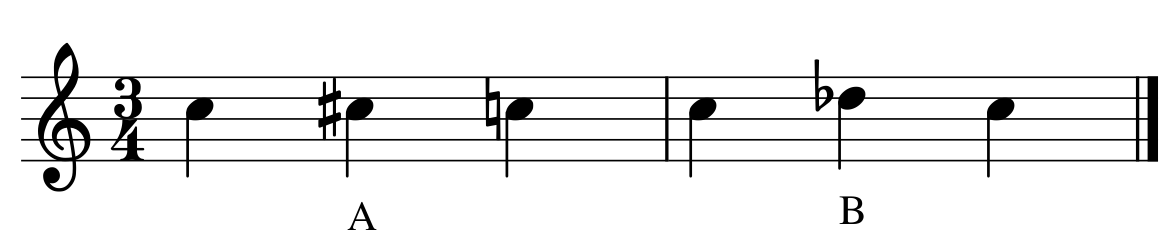
\includegraphics[width=0.8\textwidth]{figures/Q7_3.png} %
% \caption{Two notations (A and B) of a chromatic %
% neighbouring note. Regardless of the harmonic and key %
% context, the second note should probably be spelled as %
% in version B.} \label{fig:Q7_3} \end{figure}

One example of a complicated harmonic context is the
presence of a German augmented sixth, for which Teodoru and
Raphael write \parencite{teodoru2007pitch}:

\begin{italicquotes}
Other situations require a deeper notion of the harmonic
state than provided by the local key, as in the German
augmented sixth chord, which seems nearly impossible to
spell correctly without recognizing it as such.
\end{italicquotes}

Overall, designing a pitch-spelling algorithm poses
important challenges in different musical fronts, but it
also provides researchers with the opportunity of putting in
practice different analytical models (e.g., local key, chord
labeling, and non-chord detection) for solving a common
task. Furthermore, unlike many of those models which suffer
from highly ambiguous evaluations, pitch spelling presents a
simple way of assessing whether our computational models
understand the musical context or not. That is, the note is
either G$\sharp$ or A$\flat$, and there is only one right
answer.

In the following section, a survey is provided with
different pitch-spelling algorithms that have been developed
throughout the years.
